Les differentes maquettes du site permettent d'améliorer la vision des besoins de l'application.
Ces visuels ne sont pas définitifs et sont simplement là pour nous aider à mieux structurer l'application et organiser les objectifs nécessaires à la réalisation de celle-ci.
\begin{figure}[H]

\centering
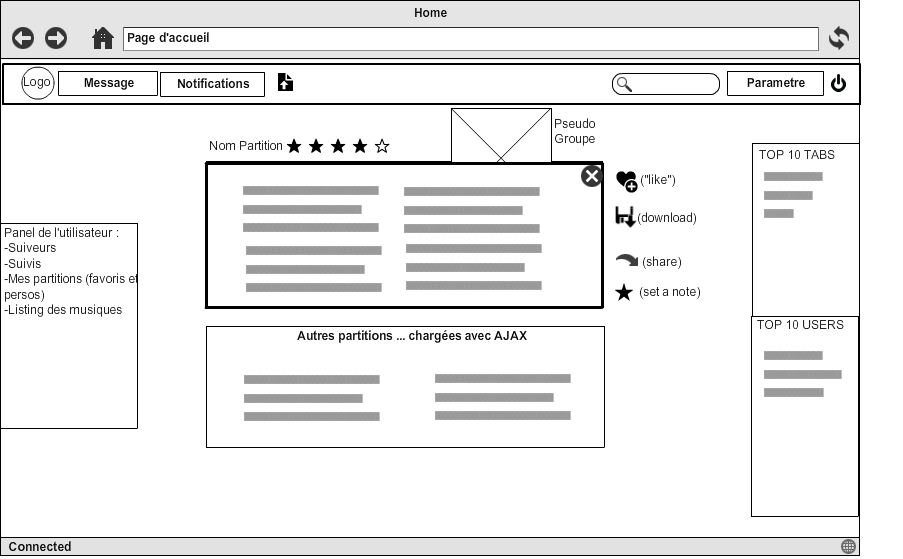
\includegraphics[scale=0.5]{Home}
\caption{Maquette de la page principale du site}
La barre du haut est une barre de menu qui sera
disponible sur toute les pages du site, elle n'est pas
représentée sur toutes les maquettes par soucis de clarté. En
effet, le principal sujet des maquettes suivantes n'est pas
la présence de la barre de menu mais le contenu de celles-ci
\end{figure}

\begin{figure}[H]

\centering
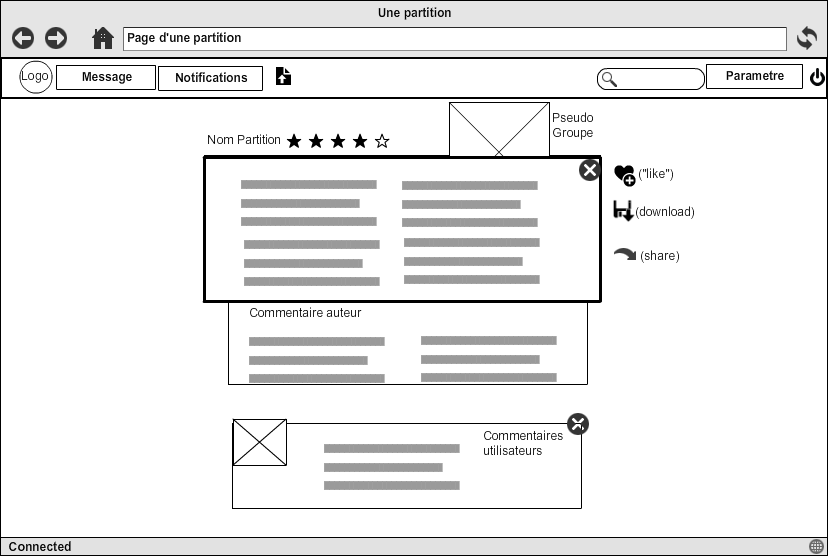
\includegraphics[scale=0.5]{Tab}
\caption{Page principale d'une partition de musique}
\end{figure}


\begin{figure}[H]

\centering
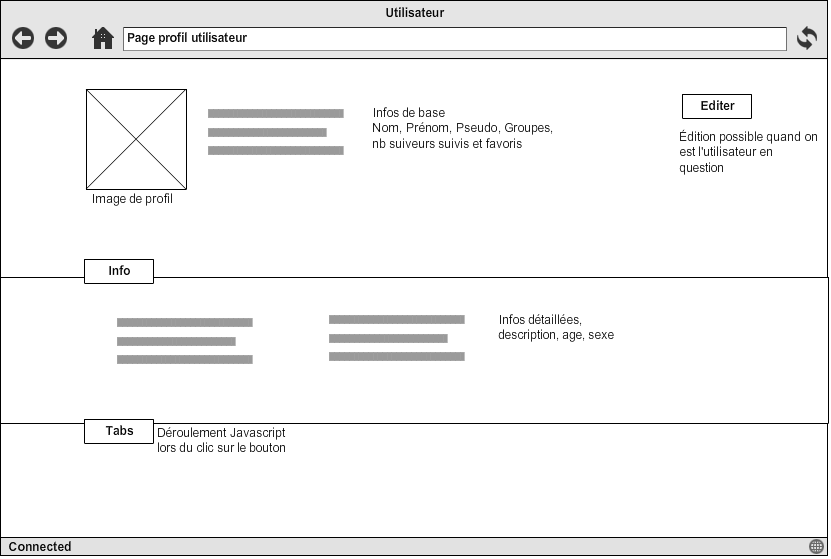
\includegraphics[scale=0.5]{User}
\caption{Page de profil utilisateur}

Cette page permettra à l'utilisateur concerné de modifier ses informations s'il le souhaite.
\newline Les autres utilisateurs verront sur sa page de profil les informations rendues visibles par l'utilisateur en question.
\end{figure}

\begin{figure}[H]

\centering
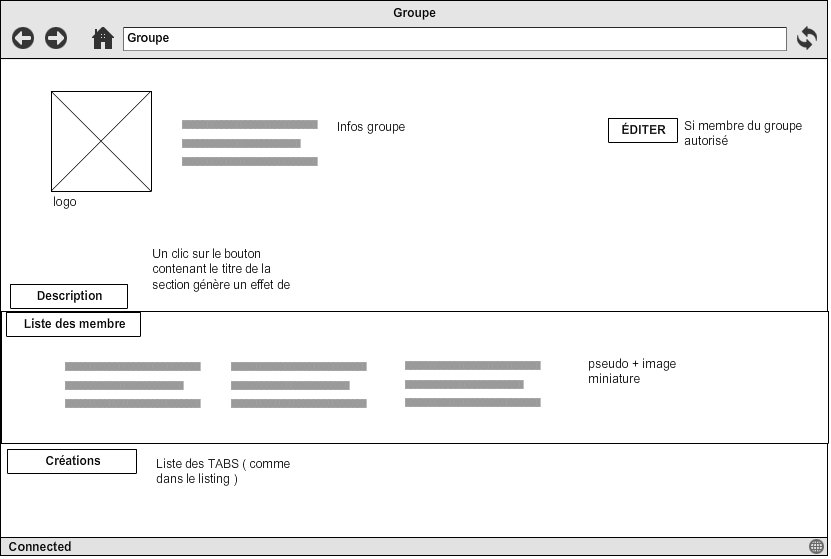
\includegraphics[scale=0.5]{Group}
\caption{Page d'un groupe de musique}

Cette page permettra de modifier le groupe si l'utilisateur en possède les droits.
\newline Cette page contiendra la liste des membres du groupe ainsi que les différentes partitions liées au groupe concerné.
\end{figure}

\begin{figure}[H]
\centering
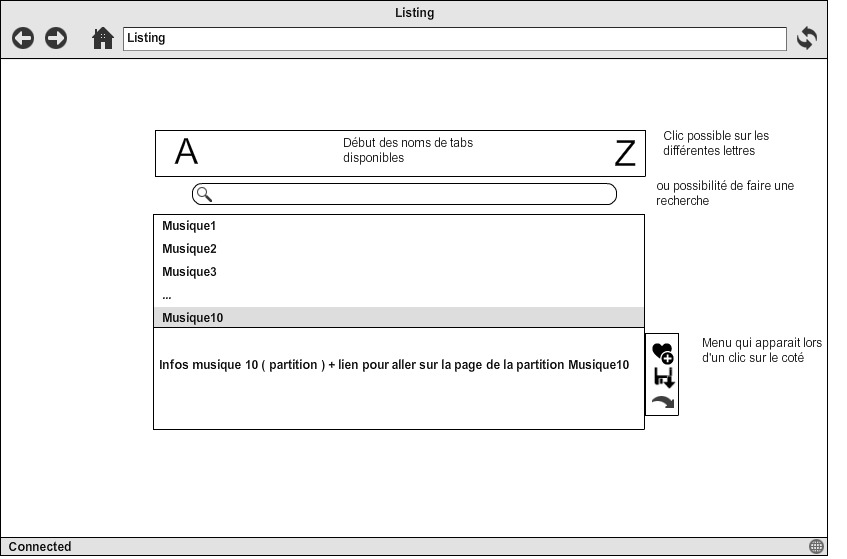
\includegraphics[scale=0.5]{Listing}
\caption{Liste de toutes les partitions}

Le listing des partitions permettra une recherche plus approfondie qu'avec la recherche disponible dans la barre de menu (la barre du haut).

\end{figure}
